 \documentclass[10pt]{beamer}
\usepackage{graphicx}
\usepackage{amsmath}
\usepackage{cite}
\usetheme{Madrid}
\usepackage{stackengine}
\usepackage{amsfonts,amsmath,amssymb}
\usepackage{multicol}
\usepackage{amsthm,amsfonts,amssymb,amsmath,graphicx}
\DeclareMathOperator*{\maxi}{maximize}
\setbeamertemplate{caption}[numbered]
\definecolor{aqua}{rgb}{0.0, 1.0, 1.0}
\usecolortheme[named=violet]{structure}
\title[]{ A Rate-Splitting Approach to the Gaussian Multiple-Access Channel}
\author[Ritesh]{\textbf{By : Ritesh Kumar} \newline Dept. of Electrical Engineering \newline (EE20RESCH11005) \newline \newline Under the supervision of	\newline \textbf{Dr. Shashank Vatedka}}
\institute{IIT Hyderabad}
\date
\today

\begin{document}
	\begin{frame}
		\titlepage
	\end{frame}
	%\tableofcontents
%	\begin{frame}[t]{INTRODUCTION}\vspace{5pt}
%		\begin{enumerate}
%			\item \textbf{ Federated Learning \cite{6}:}
%		\end{enumerate}
%		\begin{itemize}
%			\item<1-> It is a machine learning setting where the main goal is to train a high quality centralized model.
%			\item <2->In this, training data remain distributed over a large number of clients.
%			
%			\begin{figure}[htb!]   
%				\centering
%				\includegraphics[height=.25\textheight]{Fig_1.pdf}
%				\label{fig1}
%			\end{figure}
%			\item <3-> Model is updated by each client independently, based on its local training datasets and model sent by the server. 
%			\item <4->Based on the updated model sent back by clients, the server computes a new global model.
%		\end{itemize}
%	\end{frame}
	
%	\begin{frame}[t]{Statistical Parameter Estimation in Distributed Learning}\vspace{5pt}	
%		\begin{itemize}
%			\item<1->  Recently, algorithms involving distributed mean estimation have been used extensively in ML algorithms and neural networks.\vspace{10pt}
%			\begin{figure}[htb!]   
%				\centering
%				\includegraphics[height=.40\textheight]{Fig_2.1.1.pdf}
%				\label{fig2}
%			\end{figure}
%			\item <2-> We study the basic problem of finding the optimal minimax rate in distributed mean estimation with limited communication.  	
%		\end{itemize}
%	\end{frame}
%	\begin{frame}[t]{Distributed Mean Estimation with Limited Communication}
%		\begin{enumerate}
%			\item \textbf{Model }
%		\end{enumerate}
%		\begin{itemize}
%			\item <1->We have given $n$ vectors $X^{n} = X_{1}, X_{2}, X_{3}, \dots X_{n} \in \mathbb{R}^{d} $ that reside on the clients.
%			\begin{figure}[htb!]   
%				\centering
%				\includegraphics[height=.40\textheight]{Fig_2.1.pdf}
%				\label{fig3}
%			\end{figure}
%			\item <2-> The goal of distributed mean estimation is to estimate the mean of the vectors : 
%			\begin{align}
%				\bar{X} = \frac{1}{n} \sum_{\imath=1}^{n} X_{\imath} 
%			\end{align}	
%		\end{itemize}
%	\end{frame}
	
	\begin{frame}[t]{Introduction}\vspace{5pt}
		\begin{enumerate}
			\item <1->This presentation is based on the paper.\\
			\small{\textbf{ B. Rimoldi and R. Urbanke, “A rate splitting approach to the Gaussian
					multiple access channel,” IEEE Trans. Inf. Theory, vol. 42, pp. 364–375,
					Mar. 1996.}}\\
	

		\item<2-> Assumptions :
		\begin{itemize}
			\item Channel is discrete-time and frame synchronous with power constraint \begin{equation}
				P = \left( P_1, P_2 \dots P_M \right)
			\end{equation}
		Where $P_i$ is power constraint for user $i$.
			\item Noise variance is $\sigma^2$.
			\item ``code" stands for the ideal random code. And decoding scheme use successive cancellation.
			
		\end{itemize}
	
			\end{enumerate}
	\end{frame}
	
	\begin{frame}[t]{}\vspace{5pt}
		\begin{itemize}
			\item <1-> Random codes have a decoding complexity of of the order of $2^{nR_{\text{sum}}}$. 
		%	Where $R_{\text{sum}} =  R_1 + R_2 \dots +R_M$ is the sum rate and $n$ is the block length.	
	
	%\item<2-> Its capacity region is the subset of $\mathbf{R}^M$ containing rate touples $(R_1,\dots R_M)$.
	\item Rate touples component satsfying the condition
	\begin{equation}
		\sum_{i \in S}  R_i\leq \frac{1}{2}\log_2\left(1 + \frac{\sum_{i \in S} P_{i} }{\sigma^2} \right) \hspace{10pt}\forall S \subseteq \{ 1, \dots ,M\}
	\end{equation}
	 \begin{center}
	\begin{figure}[htb!]
		\centering
		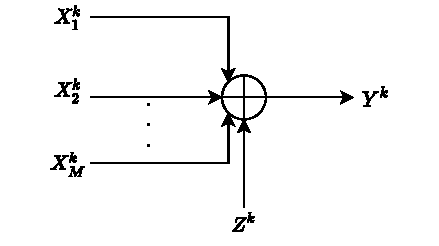
\includegraphics[height=.3\textheight]{pic1.pdf}
		\caption{Gaussian multiple-access channel}
		\label{fig1}
	\end{figure}
\end{center}
	\end{itemize}
	\end{frame}
\begin{frame}[t]{RSMA}
	\begin{itemize}
		\item RSMA is a multiple access technique in which we split the message of user in 2 parts.
			\begin{figure}[htb!]
			\centering
			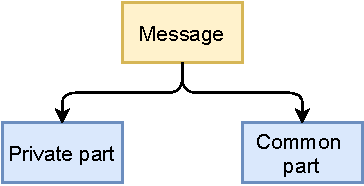
\includegraphics[height=.3\textheight]{pic_7.pdf}
			\caption{Message splitting}
			\label{fig1.1}
		\end{figure}
	\end{itemize}
	\end{frame}

%	\begin{frame}[t]{Transmitter}
%	\begin{figure}[htb!]
%		\centering
%		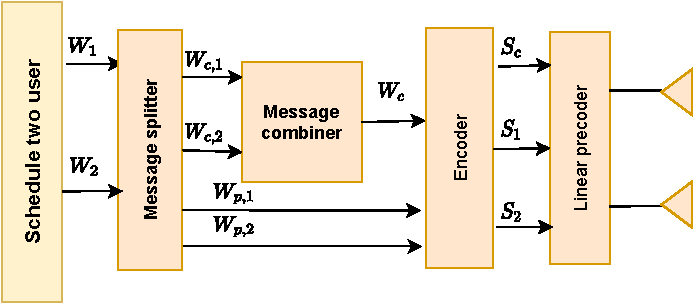
\includegraphics[height=.5\textheight]{pic_4.pdf}
%		\caption{Transmitter setup}
%		\label{fig2}
%	\end{figure}
%\end{frame}
%	\begin{frame}[t]{Receiver}
%	\begin{figure}[htb!]
%		\centering
%		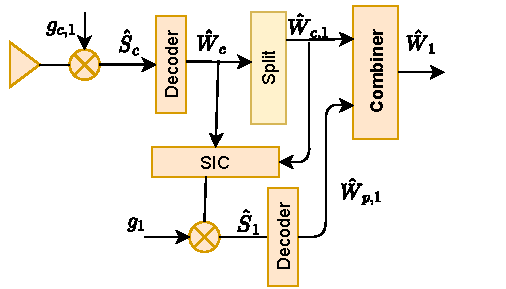
\includegraphics[height=.5\textheight]{pic_5.pdf}
%		\caption{Receiver setup}
%		\label{fig3}
%	\end{figure}
%\end{frame}
	\begin{frame}[t]{RSMA}
		\begin{figure}[htb!]
		\centering
		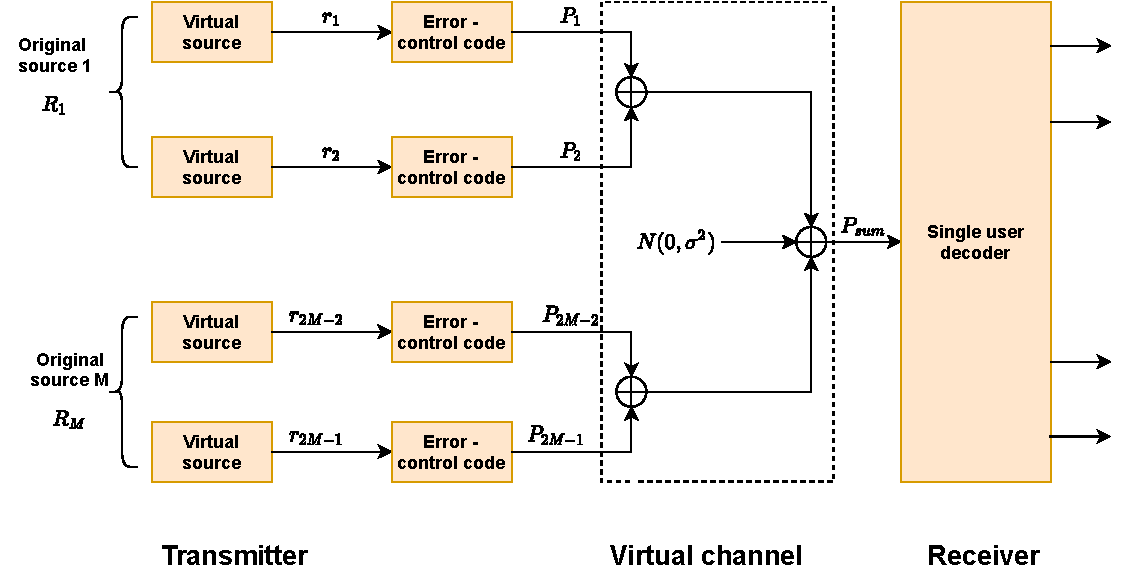
\includegraphics[height=.6\textheight]{pic_2.pdf}
		\caption{ Multiple-access system based on rate-splitting multiple accessing}
		\label{fig4}
	\end{figure}		
	\end{frame}
	\begin{frame}[t]{Single user decoding}
	\begin{figure}[htb!]
		\centering
		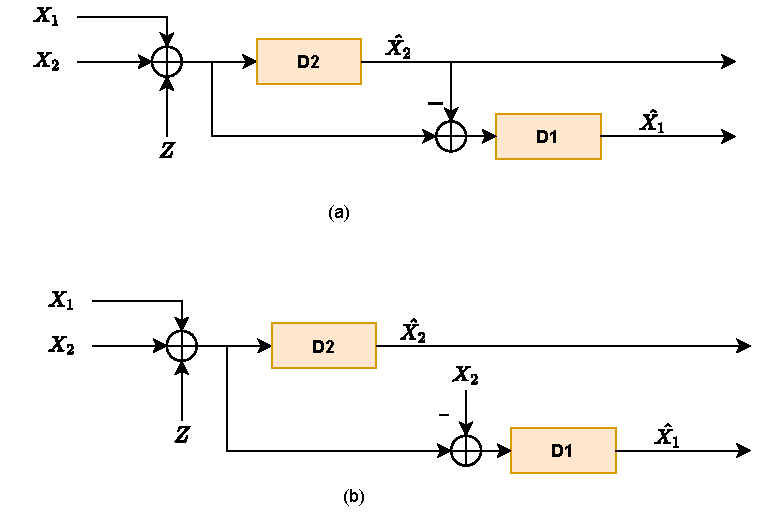
\includegraphics[height=.6\textheight]{pic_3.pdf}
		\caption{(a) Single-user decoder. (b) Genie-aided decoder}
		\label{fig5}
	\end{figure}		
\end{frame}

\begin{frame}[t]{RSMA }
\begin{itemize}
	\item One user is split into two virtual users.
	\item Let define $C(P, \sigma^2)$ as,
 \begin{equation}
		C( P, \sigma^2) = \frac{1}{2}\log_2\left( 1 + \frac{P}{\sigma^2}\right)
\end{equation}
\item With chain rule,
\begin{equation}
	C(P, \sigma^2) = C(P_1, \sigma^2) + C(P_2, \sigma^2 + P_1)
\end{equation}
\item For all nonnegative number $P_1, P_2$ and $\sigma^2$ with $P = P_1 + P_2$
\item Rate $R$ of a single user transmitting at capacity can be seen as a vertex
\begin{equation}
	\left( R_1, R_2 \right) = \left( C(P_1, \sigma^2), C(P_2, \sigma^2+P_1)\right)
\end{equation}
\item Higher rate code can be obtained from two lower rate codes.
\end{itemize}
\end{frame}

\begin{frame}[t]
	\begin{itemize}
	\item Any rate tuple $(R_1, R_2)$ in the dominant face of capacity region such that,
	\begin{align*}
	    R_1< C(P_1, \sigma^2)\\
		R_2 < C(P_2, \sigma^2) \\
		R_1+ R_2 = C(P_1 +P_2 , \sigma^2)
	\end{align*}
\item Let $\delta>0$ be the unique number wich satisfies,
\begin{equation}
	R_2 = C(P_2, \sigma^2 + \delta)
\end{equation}
\end{itemize}
\end{frame}
\begin{frame}[t]
	Now consider Gaussian MAC with noise power $\sigma^2$ and there is 3 virtual inputs.
	\begin{itemize}
		\item Power constraint is $(p_1,p_2,p_3)$ such that, 
		\begin{align*}
			p_1 = \delta\\ p_2 = P_2 \\ p_3 = P_1 -\delta
		\end{align*}
		\item Rate tuple $\left( r_1, r_2, r_3\right)$ is ,
		\begin{align*}
			r_1 = C(p_1,  \sigma^2)\\ r_2 = C (p_2, \sigma^2 +p_1) \\r_3 =C (p_2, \sigma^2 +p_1+p_2)
		\end{align*}
		\item Virtual user 2 has same rate and power constraint as the original user 2.
		\item We can also observe that,
		\begin{align*}
			r_1 +r_2 +r_3 = C(p_1+p_2 +p_3,  \sigma^2)\\  = C (P_1 +P_2, \sigma^2 ) = R_1 +R_2
		\end{align*}
	\end{itemize}
\end{frame}
\begin{frame}[t]
	\begin{figure}[htb!]
		\centering
		\includegraphics[height=.5\textheight]{fig_11.png}
		\caption{Dominant face of capacity region}
		\label{fig11}
	\end{figure}
\end{frame}
\begin{frame}[t]{Contd $\dots$}
	\begin{itemize}
		\item The geometrical relationship between $R = (R_1, R_2)$ and $r = (r1,r2,r3)$ is that, they will lie on dominant face of capacity region.
		\item Define the quardruple $\left( M, P, R, \sigma^2\right)$ and a nonnegative $\delta_i$, $i = 1, \dots , M$ that satisfies
		\begin{equation}
			R_i = C(P_i, \delta_i+\sigma^2)
		\end{equation}
	\end{itemize}
\begin{figure}[htb!]
\centering
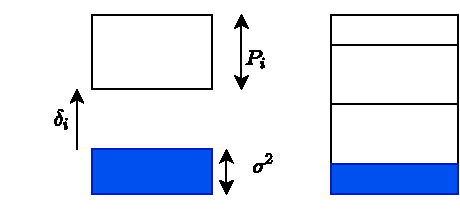
\includegraphics[height=.3\textheight]{pic_6.pdf}
\caption{Block representation}
\label{fig6}
\end{figure}
\end{frame}


\begin{frame}[t]{Lemma 1}
%	\begin{itemize}
	
\begin{block}{}
	For a tight configuration $\left(M, P, R, \sigma^2 \right)$ after a possible re-indexing, there exist at least one index $i$ for which
	\end{block}
\begin{equation}
	\delta_i \leq \delta_{i+1} \leq \delta_i  + P_i 
\end{equation}
where $\delta_i$ is a unique nonegative number that satisfies
\begin{equation}
	R_i = C(P_i, \delta_i + \sigma^2).
\end{equation}
proof:\\
	We re-index so that $ 0=\delta_0 \leq \delta_1 \leq \delta_2 \dots , \leq \delta_M $ and assume that assume that claim is false i.e., that
	\begin{equation}
		\delta_{i+1} > \delta_i + P_i, i = 0,1, \dots, (M-1)
	\end{equation}
	It follows that	
	\begin{equation}
		\sum_{i =1}^{M} R_i = \sum_{i=1}^{M} C(P_i, \sigma^2+\delta_i)<  \sum_{i=1}^{M} C \left( P_i, \sigma^2+ \sum_{j<i} P_i \right) = C \left(  \sum_{i=1}^{M} P_i, \sigma^2 \right)
	\end{equation}
	\end{frame}

\begin{frame}[t]{Lemma 2}	
	\begin{block}{}
		Consider a quardruple   $\left(M, P, R, \sigma^2 \right)$ and assume that,
		\begin{equation}
			\delta_j \geq  \delta_i + P_i \label{eq12}
		\end{equation}
		for some $i,j \in \left\{ 1,2,3 \dots, M\right\}$. Let $\delta$ be the unique nonnegative numbe such that $R_i +R_j = C(P_i + P_j, \delta )$. Then
		\begin{equation}
			\delta_i \leq \delta \leq \delta_j - P_i
		\end{equation}
	\end{block}
Proof : \\
	\begin{align*} 
 C(P_i +P_j , \delta )  = R_i + R_j =   C(P_i, \delta_i ) +  C(P_j , \delta_j )\\ \leq  C(P_i , \delta_i ) +  C(P_j , \delta_i+P_i )  =  C(P_i +P_j , \delta_i )
\end{align*}
\end{frame}
\begin{frame}[t]
From the inequality in \eqref{eq12} we can write that,
\begin{align*}
C(P_i +P_j , \delta )  = R_i + R_j =   C(P_i, \delta_i ) +  C(P_j , \delta_j )\\ \geq  C(P_i , \delta_j-P_i ) +  C(P_j , \delta_j)  =  C(P_i +P_j , \delta_j -P_i )
\end{align*}
\end{frame}
\begin{frame}[t]{Quadruple for RSMA}
The quardruple $\left(m,p,r,\sigma^2\right)$	 is a spinoff of $\left( M, P, R, \sigma^2\right)$ if there exist a surjective mapping 
$\phi : \left\{ 1, \dots, m\right\} \rightarrow \left\{ 1, \dots, M \right\}$ such that for all $i \in \left\{ 1, \dots, M\right\}$ we have,
\begin{equation*}
	P_i \geq \sum_{ j \in \phi^{-1}(i)} p_j
\end{equation*}
and,
\begin{equation*}
	R_i \leq \sum_{ j \in \phi^{-1}(i)} r_j
\end{equation*}
\end{frame}
\begin{frame}[t]{}
\begin{theorem}
	For every M-user configuration $\left(M, P, R, \sigma^2 \right)$ there exist a spinoff $\left( m,p,r, \sigma^2\right)$ which is single-user-codable.Moreover, one can guarantee that one user is un-split and that no user split into more than two virtual users. Hence $m\leq 2M-1$
\end{theorem}
%\end{block}

Proof :\\
Without loss of generality we may assume that $\left(M,P,R,\sigma^2\right)$ is tight. By induction on M we can proof this.
	\begin{itemize}
	\item for M = 1 the claim is trivially true.
	\item Consider 2 user case, i.e. M=2.
		\item Any rate tuple $(R_1, R_2)$ in the dominant face of capacity region such that,
	\begin{align*}
		R_1< C(P_1, \sigma^2)\\
		R_2 < C(P_2, \sigma^2) \\
		R_1+ R_2 = C(P_1 +P_2 , \sigma^2)
	\end{align*}
let $\delta >0 $ be a unique number such that,
\begin{equation}
	 R_2 = C(P_2 , \sigma^2 + \delta)
\end{equation}
\end{itemize}
\end{frame}
\begin{frame}[t]
Now we assume that
t it is true for an arbitrary positive M and consider the case of M+1 users.
\begin{itemize}
	\item Using lemma 1 we may assume that,
	$\delta_M \leq \delta_{M+1}$ and $\delta_{M+1}\leq \delta_M +P_M$
	\item We reduce the original (M+1) user configuration $\left(M+1, P,R, \sigma^2\right)$ to an M-user configuration $\left(M,\hat{P}, \hat{R}, \sigma^2\right)$ where,\\
	\begin{align*}	
	\hat{P_i} = P_i, i = 1,2, \dots, M-1\\
	\hat{P_M} = P_M + P_{M+1},\\   \hat{R_i} = R_i,   i = 1,2, \dots, M-1 \\  \hat{R_M} = R_M + R_{M+1}
\end{align*}
\item By induction hypothesis, there exist a spinoff $\left(m ,p, r, \sigma^2 \right)$ of $\left(M,P,R,\sigma^2 \right)$ with m $\leq$2M-1 and with property that one user is unsplit and no user is split into more than two users.
\end{itemize}
\end{frame}
\begin{frame}[t]
\begin{figure}[htb!]
	\centering
	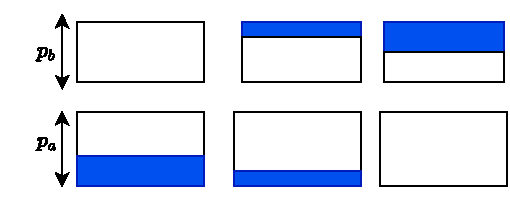
\includegraphics[height=.3\textheight]{pic_8.pdf}
	\caption{Block representation}
	\label{fig7}
\end{figure}
\end{frame}
\begin{frame}[t]
	\begin{figure}[htb!]
		\centering
		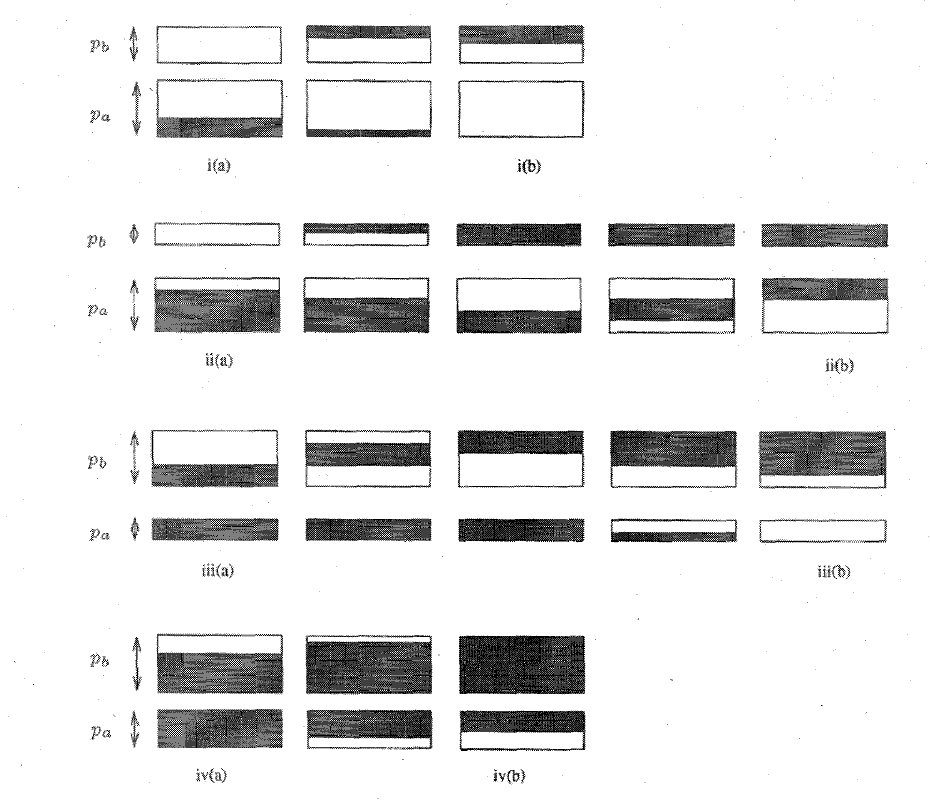
\includegraphics[height=.7\textheight]{fig_9.png}
		\caption{Block representation}
		\label{fig8}
	\end{figure}
\end{frame}
\begin{frame}[t]{Contd $\dots$}
	\begin{figure}[htb!]
		\centering
		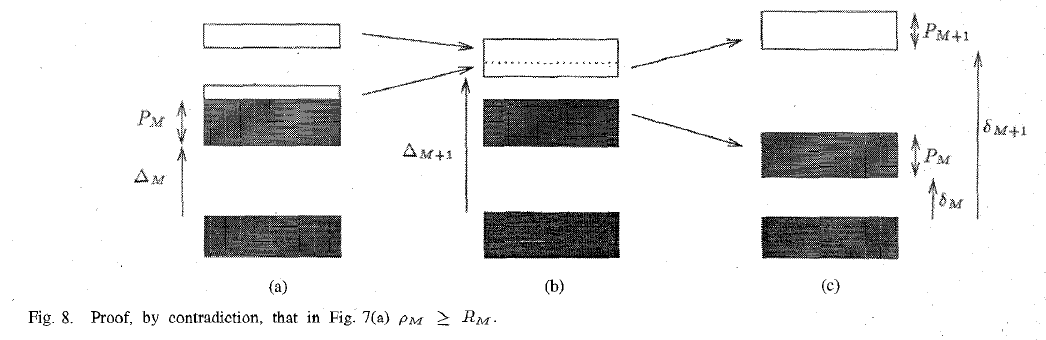
\includegraphics[height=.4\textheight]{fig_10.png}
		\caption{Block representation}
		\label{fig9}
	\end{figure}
\end{frame}

\begin{frame}[t]{Advantages of RSMA}
\begin{itemize}
	\item <1->Any point in the capacity region of a discrete-time synchronous Gaussian MAC is achievable via RSMA at relatively low coding complexity.
	\item <2-> There is no need of synchronization among users.
	\item<3-> Spread-spectrum multiple access (SSMA) has upper bound on the spectral efficiency as,
	\begin{equation}
 2R_{\text{sum}} \leq \stackunder{$\lim$}{M$\rightarrow \infty$} M\log_2\left( 1 + \frac{P}{\sigma^2 + (M-1)P}\right) = 1/log_e 2[ b/s/Hz]
  \end{equation}
\item <4-> There is no such upper bound for RSMA.
%	\item<3-> For discrete time Gaussian MAC, one can achieve rate tuples via "time-sharing" approach.
%	\item<4-> For continuous-time channel one can also do "frequency-sharing between vertices"
\end{itemize}
\end{frame}

\begin{frame}[t]
\begin{itemize}
%	\item Interference reduction resulting from intermittent transmitters.
%	\item Cellular reuse factor of 1.
	\item<1-> Channel estimation is better than narrowband system.
	\item<2-> There is no near far problem in RSMA like SSMA.
	\item<3-> RSMA allows one to achieve any point in the capacity region of a time varying multipath channel.
	\item<4-> Its allows the user to use the his extra power for the benefits of another user.
\end{itemize}
\end{frame}

\begin{frame}[t]{further research}
\begin{itemize}
	\item How RSMA behaves with the practical codes.
	\item What is the effect of the imperfect cancellation at the receiver.
	\item Effect on the Rate with various coding scheme.
\end{itemize}
\end{frame}
	\begin{frame}
	\center{\textbf{\huge{Thank You!}}}
\end{frame}	




%	\begin{frame}[t]{Stochastic Binary Quantization}
%		Consider a vector X$_{\imath}$, and 
%		\[ X_{\imath}^{\textit{max}}= \max_{ 1\leq \jmath \leq d} X_{\imath}(\jmath) \]  and, \[ X_{\imath}^{\textit{min}}= \min_{ 1\leq \jmath \leq d} X_{\imath}(\jmath) \] 
%		
%		\begin{figure}[htb!]   
%			\centering
%			\includegraphics[height=.10\textheight]{Fig_3.pdf}
%			\label{fig4.1}
%		\end{figure}
%		\begin{equation}
%			Y_{\imath}(\jmath) = \left\{\begin{matrix}
%				& X_{\imath}^{\text{max}}   \hspace{20pt}  \text{w.p.}  \hspace{20pt} \frac{X_{\imath}(\jmath) - X_{\imath}^{\text{min}}}  {X_{\imath}^{\text{max}} - X_{\imath}^{\text{min}}}\\ 
%				& X_{\imath}^{\text{min}}  \hspace{20pt}  \text{w.p.}  \hspace{20pt} \frac{ X_{\imath}^{\text{max}} - X_{\imath}(\jmath)}  {X_{\imath}^{\text{max}} - X_{\imath}^{\text{min}}} \\
%			\end{matrix}\right.
%		\end{equation}
%		\begin{itemize}
%			\item <1-> This algorithm is unbiased since $\mathbb{E}\left[\hat{x} \right] = x.$
%		\end{itemize}
%	\end{frame}
%	\begin{frame}[t]{Contd $\dots$}
%		\begin{itemize}
%			\item <1-> Total Communication cost is $C (X^{n}) \leq n.(d + O(1))$
%			\item <2->Mean square error is :
%			\begin{equation}
%				\varepsilon(X^{n}) = \mathbb{E} ||\hat{\bar{X}} - \bar{X} ||^{2}  = \frac{1}{n^{2}} \sum_{\imath = 1}^{n}\sum_{\jmath = 1}^{d} (X_{\imath}^{\text{max}} - X_{\imath}(\jmath)) (  X_{\imath}(\jmath)- X_{\imath}^{\text{min}})
%			\end{equation}
%			Since,
%			\begin{equation}
%				(X_{\imath}^{\text{max}} - X_{\imath}(\jmath)) (  X_{\imath}(\jmath)- X_{\imath}^{\text{min}}) \leq \frac{(X_{\imath}^{\text{max}} - X_{\imath}^{\text{min}})^2}{4}
%			\end{equation}
%			and,
%			\begin{equation*}
%				(X_{\imath}^{\text{max}} - X_{\imath}^{\text{min}})^2 \leq  2.|| X_{\imath}||^{2}
%			\end{equation*}
%			Hence,
%			\begin{equation}
%				\varepsilon(X^{n}) = \mathbb{E} ||\hat{\bar{X}} - \bar{X} ||^{2} \leq \frac{d}{2n}.\frac{1}{n} \sum_{\imath=1}^{n} ||  X_{\imath} ||^2 + O(1)
%			\end{equation}
%			Authors show that, this bound is tight.	
%		\end{itemize}
%		
%	\end{frame}
%	
%	
%	\begin{frame}[t]{Our Proposed Scheme }
%		\begin{block}{Lemma 1}
%			There exist an implementation of stochastic binary quantizer, that uses $ d + O(1)$    bits per client  and achieves an MSE for a given set of   vectors $X^n$ :
%			\begin{align}
%				\varepsilon (X^{n}) = \frac{1}{n}. \frac{d}{8n} \sum_{\imath=1}^{n}|| X_{\imath}||_{2}^{2}
%			\end{align}
%			
%		\end{block}
%		
%		
%		
%		\textbf{Proof :} \\
%		Consider a vector X$_{i}$, and 
%		\[ X_{\imath}^{\textit{max}}= \max_{ 1\leq \jmath \leq d} X_{\imath}(\jmath) \]  and, \[ X_{\imath}^{\textit{min}}= \min_{ 1\leq \jmath \leq d} X_{\imath}(\jmath) \] 
%	\end{frame}
%	\begin{frame}[t]{Contd $\dots$}
%		Now consider quantization a algorithm.
%%		\begin{figure}[htb!]   
%%			\centering
%%			\includegraphics[height=.20\textheight]{Fig_4.pdf}
%%			\label{fig4}
%%		\end{figure} 
%		
%		\begin{equation}
%			Y_{\imath}(\jmath) = \left\{\begin{matrix}
%				& \frac{3X_{\imath}^{\text{max}}+X_{\imath}^{\text{min}}}{4} \hspace{20pt}   \text{w.p.} \hspace{20pt} \frac{X_{\imath}(\jmath) - X_{\imath}^{\text{min}}}  {X_{\imath}^{\text{max}} - X_{\imath}^{\text{min}}}\\
%				& \frac{X_{\imath}^{\text{max}}+ 3X_{\imath}^{\text{min}}}{4} \hspace{20pt}   \text{w.p.}  \hspace{20pt} \frac{ X_{\imath}^{\text{max}} - X_{\imath}(\jmath)}  {X_{\imath}^{\text{max}} - X_{\imath}^{\text{min}}} \\
%			\end{matrix}\right.
%			\label{eq1.14}
%		\end{equation}
%		\begin{itemize}
%			\item <1-> This algorithm is biased, since $\mathbb{E}\left[ \hat{x}\right] \neq x$. And it is given as :
%		\end{itemize}
%		\begin{equation*}
%			\mathbb{E}\left[ \hat{x} \right] = \frac{2x +x_{max} + x_{min}}{4}
%		\end{equation*}
%	\end{frame}
%	
%	\begin{frame}[t]{Contd $\dots$}
%		\begin{align}
%			\varepsilon (X^{n}) = \mathbb{E} ||  \hat{\bar{X}} - \bar{X} ||^{2}_{2} = \frac{1}{n^2} \mathbb{E}|| \sum_{\jmath = 1}^{n} (Y_{\imath} - X_{\imath})||^{2}_{2} = \frac{1}{n^2} \sum_{\imath = 1}^{n} \mathbb{E} || Y_{\imath} - X_{\imath} ||^{2}_{2} 
%			\label{eq4}
%		\end{align}
%		For simplicity of calculation consider single  bit for each user in \ref{eq4}: 
%		\begin{align}
%			\mathbb{E} || Y_{\imath} - X_{\imath} ||^{2}_{2} = [ (X_{\imath} - (\frac{3X_{\imath}^{\text{max}}+X_{\imath}^{\text{min}}}{4}))^2 \alpha + (X_{\imath} - (\frac{X_{\imath}^{\text{max}}+3X_{\imath}^{\text{min}}}{4}))^2 (1 -\alpha)]  
%			\label{eq5}
%		\end{align}
%		\begin{equation*}
%			\mathop{max}_{x_{min} \leq x_{i} \leq x_{max}}  \vspace{2pt}\mathop{min}_{0 \leq \alpha \leq 1} \varepsilon (X^{n}) = \mathbb{E} || Y_{\imath} - X_{\imath} ||^{2}_{2}
%		\end{equation*}
%		Where $\alpha$= $\frac{X_{\imath}(\jmath) - X_{\imath}^{\text{min}}}  {X_{\imath}^{\text{max}} - X_{\imath}^{\text{min}}}.$
%		After solving the equation (\ref{eq5}), we got the bound as :
%		
%		\begin{align}
%			\mathbb{E} || Y_{\imath} - X_{\imath} ||^{2}_{2} \leq \frac{(X^{\text{max}} - X^{\text{min}})^2}{16}
%			\label{eq6}
%		\end{align}
%	\end{frame}
%	
%	\begin{frame}[t]{Contd $\dots$}
%		Generalizing it for n clients having each datasets of size d. 
%		The upper bound of squared for  this scheme is given as :\\
%		Using (\ref{eq6}) in (\ref{eq4}) and solving it, we got
%		\begin{align}
%			\varepsilon (X^{n}) = \frac{1}{n^2} \sum_{\imath=1}^{n}\sum_{\jmath=1}^{d} \frac{(X^{\text{max}} - X^{\text{min}})^2}{16}
%		\end{align}
%		Since, 
%		\begin{align}
%			(X_{\imath}^{\text{max}} - X_{\imath}^{\text{min}})^2 \leq 2 || X_{\imath}||_{2}^{2}
%			\label{21}
%		\end{align} 
%		We have  squared error for our  proposed scheme is :
%		\begin{align}
%			\varepsilon (X^{n}) = \frac{1}{n}. \frac{d}{8n} \sum_{i=1}^{n}|| X_{\imath}||_{2}^{2} + O(1)
%		\end{align}
%		Hence proposed scheme is   4 times more efficient than binary quantization scheme proposed by authors.
%	\end{frame}
%	
%	\begin{frame}[t]{Stochastic k-level quantization}
%		\begin{itemize}
%			\item <1-> This is generalization of binary quantization.
%			\item <2-> For every integer r $\in [0,k)$
%			\begin{equation*}
%				B_{i}(r)  = X_{\imath}^{\text{min}} + \frac{r.s_{\imath}}{k-1}, 	
%			\end{equation*}
%			Where, $s_{i} = X_{\imath}^{max} - X_{\imath}^{min}$
%			
%			\begin{equation}
%				Y_{\imath}(\jmath) = \left\{\begin{matrix}
%					& B_{\imath}(r+1)   \hspace{20pt}  \text{w.p.}  \hspace{20pt} \frac{X_{\imath}(\jmath) - B_{\imath}(r)}{B_{\imath}(r+1) - B_{\imath}(r)}\\ \\
%					&  B_{\imath}(r)   \hspace{20pt}  \text{w.p.}  \hspace{20pt} \frac{ B_{\imath}(r+1) - X_{\imath}(\jmath)}{B_{\imath}(r+1) - B_{\imath}(r)} \\
%				\end{matrix}\right.
%			\end{equation}
%			\vspace{10pt}
%			\item <3->Communication cost is $C(X^n) \leq n (d \left \lceil   log_{2}k\right \rceil + O(1))$
%		\end{itemize}
%	\end{frame}
%	
%	\begin{frame}[t]{Contd $\dots$}
%		\begin{itemize}
%			\item <1-> If $(X_{\imath}^{\text{max}} - X_{\imath}^{\text{min}})  \leq s_{\imath} \leq  \sqrt{2}.|| X_{\imath}||$ then,
%			\begin{equation*}
%				\varepsilon (X^{n}) \leq \frac{d}{2n (k-1)^2}. \frac{1}{n} \sum_{\imath=1}^{n}|| X_{\imath}||_{2}^{2}
%			\end{equation*}
%			If we use the quantization method describe in \textbf{lemma 1}, we can have more tightly bound as :
%			\begin{equation}
%				\varepsilon (X^{n}) \leq \frac{d}{8n (k-1)^2}. \frac{1}{n} \sum_{\imath=1}^{n}|| X_{\imath}||_{2}^{2}
%			\end{equation}
%		\end{itemize}
%	\end{frame}
%	\begin{frame}[t]{Stochastic Rotated Quantization}
%		\begin{enumerate}
%			\item<1->  MSE will be smaller in all above cases, if we  reduce the $(X_{\imath}^{\text{max}} - X_{\imath}^{\text{min}})$.
%			\item <2-> With the help of random rotation, we can reduce the error in the order of $O(\frac{log(d)}{n})$.
%			\item <3-> With the help of shared randomness, all clients and central servers generate a random rotation matrix according to some know distribution \textbf{R}. 
%			\begin{equation}
%				Z_{\imath} = RX_{\imath} \hspace{10pt} \text{and,} \hspace{10pt}\bar{Z} = R \bar{X}
%			\end{equation}
%			\item <4->Clients quantize the vectors \textbf{$Z_{\imath}$} instead of $X_{\imath}$
%			\item <5-> The server estimates $\bar{X}$ as :
%			\begin{equation}
%				\hat{\bar{X}} = R^{-1} \hat{\bar{Z}} , \hspace{10pt} \hat{\bar{Z}} = \frac{1}{n}\sum_{\imath = 1}^{n} \mathit{f} (Y_{\imath})
%			\end{equation}
%		\end{enumerate}
%		
%	\end{frame}
%	
%	\begin{frame}[t]{Contd $\dots$}
%		\begin{itemize}
%			\item<1-> MSE is bounded as :
%			\begin{equation}
%				\varepsilon (X^{n}) \leq \frac{d}{8n (k-1)^2}. \frac{1}{n} \sum_{\imath=1}^{n}\mathbb{E}_{R} \left[(Z_{\imath}^{\text{max}})^2 + (Z_{\imath}^{\text{min}})^2 \right]
%				\label{18}
%			\end{equation} 
%			Where $Z_{\imath} = RX_{\imath}$ and $s_{\imath} = Z_{\imath}^{\text{max}} - Z_{\imath}^{\text{min}}$
%			
%			\item <2->In this case $R$ is a special type of matrix defined as :
%			\begin{equation*}
%				R = HD
%			\end{equation*}
%			Where,
%			\begin{itemize}
%				\item $D$ is random diagonal matrix with i.i.d. Rademacher entries.
%				\item $ H $ is Walsh-Hadamard matrix. 
%			\end{itemize}
%			
%		\end{itemize}
%	\end{frame}
%	\begin{frame}[t]{Contd $\dots$}
%		\begin{itemize}
%			\item <1->The value of $ \mathbb{E} \left[  Z_{\imath}^{min} \right]$ and $ \mathbb{E} \left[  Z_{\imath}^{max} \right]$ is bounded as :
%			\begin{equation}
%				\mathbb{E} \left[  (Z_{\imath}^{min})^2 \right] = \mathbb{E} \left[ ( Z_{\imath}^{max})^2 \right] \leq  \frac{|| X_{\imath} ||_{2}^{2} (2log \hspace{1pt}d + 2)}{d}
%			\end{equation}
%			\item <2->Using this in equation \ref{18}, we get a bound as :
%			\begin{equation}
%				\varepsilon (X^{n}) \leq \frac{ (2log \hspace{1pt}d + 2)}{4n (k-1)^2}. \frac{1}{n} \sum_{\imath = 1}^{n}|| X_{\imath}||_{2}^{2}
%			\end{equation}
%			\item <3->Communication cost is $C(X^n) \leq n (d ( \left \lceil   log_{2}k + \right \rceil + 1 ) + O(1))$	
%		\end{itemize}
%	\end{frame}
%	\begin{frame}[t]{Variable Length Coding}
%		\begin{enumerate}
%			\item  Using this, we can reduce the communication cost.
%			\item This can be use in k-level quantization technique.
%			\begin{itemize}
%				\item <1-> To encode $Y_{\imath}$ authors were initially using $d \left \lceil  log_{2} \hspace{1pt}k  \right \rceil$ bits.
%				\item <2-> Now, instead of this, they encode $h_{r}$ the number of times each quantized value $r$ appeared.
%				\item <3-> Use arithmetic or Huffman coding to encodes  with probability distribution as $p_{r} = \frac{h_r}{d}$.
%			\end{itemize}
%			\item <4->Communication cost is given as :
%			\begin{equation}
%				C(X^{n}) = n(d(2+ log_{2} \hspace{1pt}(\frac{(k-1)^2}{2d})) + k.log_{2} \hspace{1pt} \frac{(d
%					+k)e}{k} + O(1))
%			\end{equation}
%		\end{enumerate}
%	\end{frame}
%	
%	\begin{frame}[t]{Contd $\dots$}
%		\small{
%			\begin{table}[htb!]\vspace{10pt}
%				\begin{center} 
%					\caption{\tiny{Summary of the results by A. T. Suresh et al. \cite{7}}}
%				\end{center}
%				\label{ tab:1} 
%				\centering
%				\begin{tabular}{|p{2.5cm}|p{4cm}|p{4cm}|}%\vspace{10pt}
%					\hline			
%					\textbf{Algorithm } &  \textbf{Cost } & \textbf{ MSE} \\ 
%					\hline
%					Stochastic uniform quantization & \small{ $C(X^n) = n.(d + O(1)) $} & $  \varepsilon(X^n)  \newline = \theta(\frac{d}{n}.\frac{1}{n}\sum_{\imath=1}^n||X_\imath||_2^2) $ \\
%					\hline
%					Stochastic K-level quantization & \small{ $C(X^n) = n.(d  \left \lceil log_{2}k \right \rceil  + O(1)) $ } & $ \varepsilon(\pi_{sk},X^n)  \newline = O(\frac{d}{n(k-1)^2}.\frac{1}{n}\sum_{\imath=1}^n||X_\imath||_2^2)$ \\
%					\hline
%					Stochastic rotated quantization & \small{ $ C(X^n) = n.(d ( \left \lceil log_{2}k \right \rceil + 1 ) + O(1)) $} &  $\varepsilon(\pi_{srk},X^n)  \newline = O(\frac{\log d}{n(k-1)^2}.\frac{1}{n}\sum_{\imath=1}^n||X_\imath||_2^2)$ \\
%					\hline
%					Variable length coding & \small{ $C(X^n) = O(nd(1+ log(k^2 / d +1 ) +(\hat{O}(n)) )$} & $ \varepsilon(\pi_{svk},X^n) \newline = O(\frac{1}{n}.\frac{1}{n}\sum_{\imath=1}^n||X_\imath||_2^2) $ \\
%					\hline
%				\end{tabular} 	
%			\end{table}
%		}
%	\end{frame}
%	\begin{frame}
%		\center{\textbf{\huge{Sharing a real number}}}
%	\end{frame}	
	
%	\begin{frame}[t]{Sending a Real number [0,1]}
%		\begin{enumerate}
%			\item <1-> Consider the single-bit quantization problem.\vspace{20pt}
%			
%			
%			\begin{figure}[htb!]   
%				\centering
%				\includegraphics[height=.50\textheight]{Fig_5.pdf}
%				\label{fig5}
%			\end{figure}
%		\end{enumerate}
%	\end{frame}
%%	
%%	\begin{frame}[t]{Contd $\dots$}
%		\begin{figure}[htb!]   
%			\centering
%			\includegraphics[height=.5\textheight]{Fig_7.pdf}
%			\label{fig6}
%		\end{figure}
%	\end{frame}
%	
%	\begin{frame}[t]{Randomized Rounding}
%		\begin{itemize}
%			\item <1-> Sender uses private randomness to generate $X$ $\sim$Bernoulli(x) which is sent using a single bit.
%			\begin{equation}
%				X = \left\{\begin{matrix}
%					1 & \text{with probability $x$}\\ 
%					0  & \text{with probability (1-x)}\\
%				\end{matrix}\right.
%			\end{equation}
%			
%			\item <2->Receiver estimates $\hat{x}$ from the received $X$.
%			
%			
%			\item <3->Since $X$ is generated from Ber(x), Hence, \\
%			\begin{align*}
%				\mathbb{E} \left[ X \right]  = p(X = 0).0 + p(X = 1).1 \\
%				\implies \mathbb{E} \left[ X \right] = (1-x).0 + x.1 = x \\
%				\implies \mathbb{E} \left[ X \right] = x \hspace{5pt}\text{and,} \\
%				\implies  \mathbb{E} \left[ X \right] = \mathbb{E} \left[ \hat{x} \right] = x \\
%			\end{align*}
%		\end{itemize}
%	\end{frame}
%	\begin{frame}[t]{Contd $\dots$}
%		\begin{itemize}
%			\item  \textbf{Mean Square Error (MSE):}
%		\end{itemize}
%		\begin{align*}
%			\mathbb{E} \left [(x- \hat{x})^2 \right ] = p(X=0).(x-0)^2 + p(X=1)(x-1)^2 
%		\end{align*}
%		\begin{align*}
%			\implies \mathbb{E} \left [(x- \hat{x})^2 \right ] = (1-x).x
%		\end{align*}
%		Maximizing it to get upper bound with x, we got,\\
%		\begin{align*}
%			\implies \mathbb{E} \left [(x- \hat{x})^2 \right ] \leq \frac{1}{4}
%		\end{align*}
%		
%	\end{frame}
%	
%	\begin{frame}[t]{Deterministic Rounding}
%		\begin{itemize}
%			\item <1->With deterministic rounding, Sender sends $X = 1$ when x $\geq$ 1/2.
%			\item <2->Receiver estimate $\hat{x}$ as :
%			\begin{align}
%				\hat{x} = \frac{X}{4} + \frac{1}{4}
%			\end{align}
%			\item <3->This is not an unbiased estimator.
%			\item <4->Deterministic rounding has an (absolute) error of at most 1/4,
%			\item <5->Any deterministic biased scheme achieves worst-case expected squared error of at least 1/16 \cite{8}.
%		\end{itemize}
%	\end{frame}
	
%	\begin{frame}[t]{Algorithm with Shared Randomness}
%		\begin{figure}[htb!]   
%			\centering
%			\includegraphics[height=.50\textheight]{Fig_9.pdf}
%			\label{fig11}
%		\end{figure}
%	\end{frame}	
	
	
	
%	\begin{frame}[t]{3. Lower Bounds for x $\in$ $\left [ 0, 1\right ]$ Unbounded shared randomness.}
%		\begin{itemize}
%			\item <1-> Assume sender and receiver have access to shared randomness h .
%			\item <2->Shared randomness as a uniformly random point (s,t) from the disk with radius 1/2 and center (1/2,0).
%			
%			
%			\begin{equation}
%				X = \left\{\begin{matrix}
%					1  & \text{if} & x \geq s\\
%					0 & else
%				\end{matrix}\right.
%			\end{equation}
%			\item <3->Estimator estimates x as :
%			\begin{equation}
%				\hat{x} = \left\{\begin{matrix}
%					\frac{1}{2} - \frac{\pi}{8} \sqrt{\frac{(1-s)}{s}}  & \text{if} & X = 0\\
%					\frac{1}{2} + \frac{\pi}{8} \sqrt{\frac{s}{(1-s)}}  & \text{if} & X = 1\\
%				\end{matrix}\right.
%			\end{equation}
%			Where pdf of s is,
%			\begin{equation}
%				f(s) = \frac{8}{\pi} \sqrt{s(1-s)}
%			\end{equation}
%		\end{itemize}
%	\end{frame}
%	\begin{frame}[t]{Contd $\dots$}
%		
%		$	
%		\mathbb{E}\left[\hat{x}  \right] =	\int_{0}^{x} \left( \frac{1}{2} + \frac{\pi}{8} \sqrt{\frac{s}{1-s}} \right)  
%		\frac{8}{\pi} \sqrt{s(1-s)} ds $		
%		$ + \int_{x}^{1} \left( \frac{1}{2} - \frac{\pi}{8} \sqrt{\frac{1-s}{s}} \right)  
%		\frac{8}{\pi} \sqrt{s(1-s)} ds 
%		$		
%		\begin{equation}
%			\mathbb{E} \left[\hat{x} \right]=  \int_{0}^{1} \frac{4}{\pi} \left(  \sqrt{s(1-s) +} + s \right) ds - \int_{x}^{1} 1.ds = x
%		\end{equation}	
%		
%		
%		
%		\begin{itemize}
%			\item<1-> Estimator of this algorithm is unbiased since, $\mathbb{E}[\hat{x}] = x $
%			\item <2->Variance is bounded as :
%			\begin{equation}
%				Var[\hat{x}] \geq \frac{\pi^{2}}{64} - \frac{1}{12} 
%			\end{equation}
%		\end{itemize}
%	\end{frame}
%	
%	\begin{frame}[t]{1.$\ell$-bit shared randomness and unbounded private randomness.} 
%		\begin{itemize}
%			\item<1-> Shared randomness is limited to $\ell$ bits.
%			\item <2->Sender uses unbounded private randomness r $\sim$ U[0, 1].
%			\begin{equation}
%				X = \left\{\begin{matrix}
%					1 & \text{if} &  x \geq (r+h)2^{-\ell}\\ 
%					0  & \text{otherwise}\\
%				\end{matrix}\right.
%			\end{equation}
%			\item <3-> Receiver estimates $X$ as:
%			\begin{equation}
%				\hat{x} = X + (h - 0.5(2^\ell -1)).2^{-\ell}
%			\end{equation}
%			\item <4->This estimator is unbiased, hence MSE is given by \cite{8}.
%			\begin{equation}
%				Var[\hat{x}] \leq 1/12 . (1 - 4^{-\ell}) + 1/4.(4^{-\ell}) = 1/6(1/2 + 4^{-\ell})
%			\end{equation}
%			
%		\end{itemize}
%	\end{frame}
	%\begin{frame}[t]{Contd $\dots$}
	%	\textbf{The x $\in \{ 0, 1/2, 1\}$ case :}
	%	\begin{itemize}
	%		\item In this case we we do not require the private randomness as we can rewrite algorithm as:
	%		\begin{equation}
	%			X = \left\{\begin{matrix}
	%				0 & \text{if} &  x = 0\\ 
	%				1 - h & \text{if} & x = 1/2\\
	%				1 & \text{if} & x = 1
	%			\end{matrix}\right.
	%		\end{equation}
	%	\item Estimator estimates as :
	%\begin{equation}
	%	\hat{x} = X + \frac{(h - (1/2))}{2}
	%\end{equation}
	%		
	%		
	%		\item  For $\ell$ = 1 bit algorithm gives Var$\left[ \hat{x}\right] = 1/16$. 
	%	\end{itemize}
	%\end{frame}
	
	%\begin{frame}[t]{Contd $\dots$}
	%	\begin{itemize}
	%		\item \textbf{ If estimator is Biased :}
	%		Sender sent X as :
	%	\begin{equation}
	%		X = \left\{\begin{matrix}
	%			1  & \text{if} & x = 1 & \text{or} & (x = 1/2 & \text{and} & h = 0)\\
	%		0 & else
	%		\end{matrix}\right.
	%	\end{equation}
	%		\begin{itemize}
	%			\item <1->We need to share single bit of randomness as h $\in$ $\{0,1\}$. 
	%			\item <2->For some $\alpha$ $\in$   $\left[ 0,1\right]$ estimator estimate $\hat{x}$ as :
	%			\begin{equation}
	%				\hat{x} = \alpha .h + (1- \alpha) X.
	%			\end{equation}
	%		\end{itemize}
	%	\end{itemize}
	%
	%\end{frame}
	
%	\begin{frame}[t]{2. $\ell$-bit shared randomness $\&$ No private randomness}
%		
%		
%		\begin{itemize}
%			\item <1->Sender sends X as :
%			\begin{equation}
%				X = \left\{\begin{matrix}
%					1  & \text{if} &  x \geq T(h)\\
%					0 & else
%				\end{matrix}\right.
%			\end{equation} 
%			Where $T(h) = ah +b $ is some threshold.
%			\item<2-> \begin{equation}
%				X = \left\{\begin{matrix}
%					1  & \text{if} & x \geq 0.4 + 0.2h\\
%					0 & else
%				\end{matrix}\right.
%			\end{equation}
%			\item<2->  For some value of $\alpha$ $\in \left[0,1\right]$ estimator estimates x as :
%			\begin{equation}
%				\hat{x} = Z(\alpha).h+ Y(\alpha)X
%			\end{equation} 
%			\begin{equation}
%				\hat{x} = 0.1 + 0.2h+ 0.6X
%			\end{equation}
%			%\item <3->If h $\in$ $\left\{0,1\right\}$ then we get a cost of $1/20$. 
%			\item <4-> If $\ell$ = 4 bits, cost  becomes $\approx$ 0.04611. For $\ell$ = 8 bits, then its becomes $\approx$ 0.04599
%		\end{itemize}	 	
%	\end{frame}
%	
%	
%	\begin{frame}[t]{Contd $\dots$}
%		\small
%		{
%			\begin{table}[htb!]\vspace{10pt}
%				\centering	 	
%				\caption{\small{State of art for 1-bit quantization (Ben-Bast et al.)}}
%				%	\label{ tab:2} 
%				\begin{tabular}{|p{4cm}|p{3cm}|p{3cm}|}%\vspace{10pt}
%					\hline		
%					\textbf{Algorithm } &  \textbf{With Unbiased Estimator ( Variance ) } & \textbf{ Biased ( Expected Square error ) } \\ \hline
%					
%					No shared randomness &  $\frac{1}{4}$ ( With randomized rounding ) &  $\frac{1}{16}$ ( Deterministic rounding ) \\
%					\hline 
%					Lower Bounds for $ x \in [0, 1]$ Unbounded shared randomness  & $ \frac{\pi^{2}}{64} - \frac{1}{12} \approx 0.0708$ & $\approx 0.0459 $ \\
%					\hline
%					$\ell$-bit shared randomness with unbounded private randomness &   $ \ell = 1 : \frac{1}{8} = 0.125,  \ell = 8 : \approx 0.08334 $ \hspace{5mm} In general : $\frac{1}{6}.(\frac{1}{2} + 4^{-\ell} )$  & Open  \\
%					\hline
%					$\ell$-bit  shared randomness no private  randomness &  Impossible &  $ \ell = 1:\frac{1}{20 } = 0.05
%					, \ell =8 :\approx 0.04599$  \\
%					\hline
%				\end{tabular}
%				\label{tab:2}  
%			\end{table}
%		}
%	\end{frame}
%	
%
%	
	
	
	
	
	
	
	
\end{document}